Die drei Grundschaltungen des Transistors werden nach dem der Ausgangs- und
Eingangsspannung gemeinsamen Potential benannt. Demnach existieren Emitter-,
Kollektor- und Basisschaltung. Zum Entfernen der Gleichanteile des Ein- und
Ausgangssignals werden Kondensatoren vor die Eingänge geschaltet, welche so
dimensioniert sind, dass sie für die Wechselanteile der Signale einen
Kurzschluss darstellen.

Bei der Arbeitspunkeinstellung werden die Kondensatoren entfernt und die
Widerstände im gewünschten Arbeitspunkt ($I_C, U_{CE}$) ermittelt.

\subsubsection{Emitterschaltung}

\begin{figure}[H]
  \begin{center}
    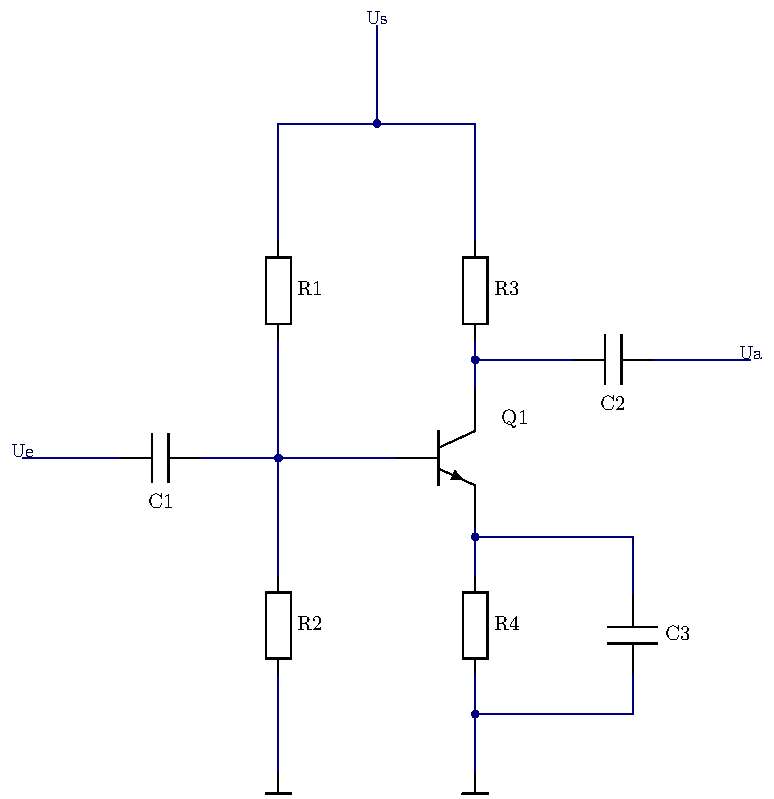
\includegraphics[width=0.618\textwidth]{circuits/commonEmitter.pdf}
  \end{center}
  \caption{Emitterschaltung}
\end{figure}

Mithilfe der Stromgegenkopplung durch den Widerstand $R_4$ lässt sich der
Arbeitspunkt gegenüber Änderungen der Stromverstärkung stabilisieren, er
verringert jedoch die Verstärkung und erhöht den Eingangs- und Ausgangswiderstand.
Man kann einen Kondensator ($C_3$) parallel schalten, um die negative Auswirkung
des Widerstands für Wechselsignale zu unterdrücken. Allgemein besitzt die
Emitterschaltung eine hohe Spannungsverstärkung sowie einen hohen Ein- und
Ausgangswiderstand.

\subsubsection{Kollektorschaltung (Emitterfolger)}
\begin{figure}[H]
  \begin{center}
    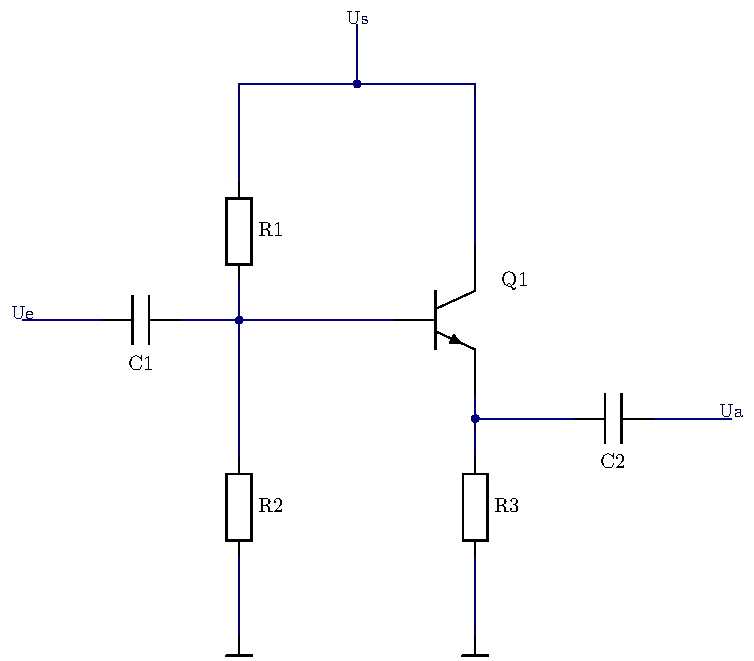
\includegraphics[width=0.618\textwidth]{circuits/commonCollector.pdf}
  \end{center}
  \caption{Kollektorschaltung}
\end{figure}

Das Ausgangsspannungssignal der Kollektorschaltung folgt etwa dem Eingangssignal
($-0.7\,\si{\volt}$), die Spannungsverstärkung ist $1$, der Ausgangsstrom ist
jedoch deutlich höher als der Eingangsstrom. Der Eingangswiderstand
der Schaltung ist daher sehr hoch, der Ausgangswiderstand ist umgekehrt proportional
der Steilheit des Transistors, also in der Regel sehr gering, weshalb sich die
Schaltung gut als Impedanzwandler eignet. 

Die Arbeitspunkteinstellung ist analog der Arbeitspunkteinstellung bei der Emitterschaltung.
Zusätzlich kann, wie bei der Emitterschaltung, ein Kollektorwiderstand
eingeführt werden, welcher dann über einen, ebenfalls zusätzlichen, vom
Kollektor an Masse
geführten Kondensator wechselspannungsmäßig kurzgeschlossen wird.

\[R_{ein} \approx r_\pi (1 + g_m \cdot R_3)\]
\[R_{aus} \approx \frac{1}{g_m}\]

\subsubsection{Basisschaltung}
\begin{figure}[H]
  \begin{center}
    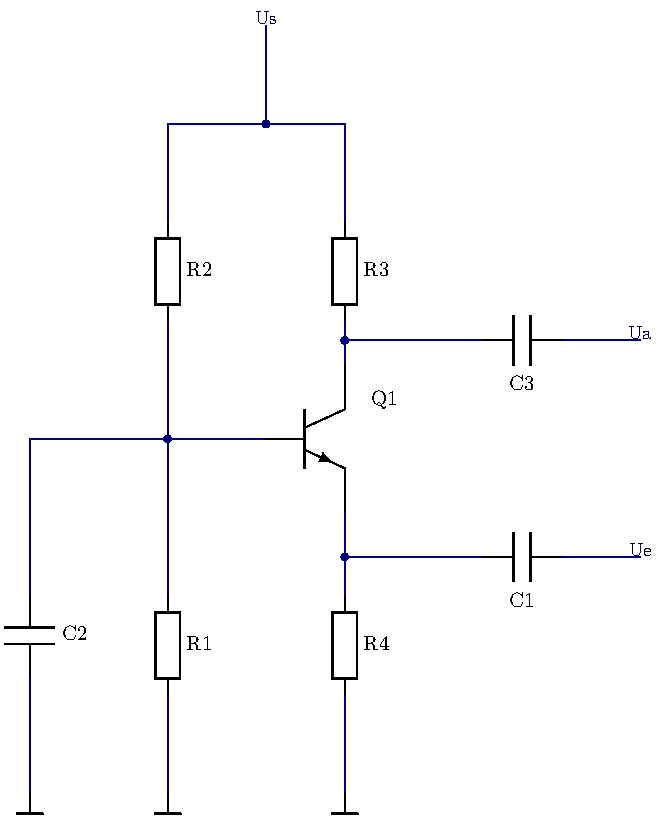
\includegraphics[width=0.618\textwidth]{circuits/commonBase.pdf}
  \end{center}
  \caption{Basisschaltung}
\end{figure}

Die Basisschaltung kennzeichnet sich durch einen sehr geringen
Eingangswiderstand, einen hohen Ausgangswiderstand sowie eine hohe Spannungsverstärkung.
Auch hier geschieht die Arbeitspunkteinstellung über das 4-Widerstandsnetzwerk
aus $R_2, R_1, R_3$ und $R_4$. Der Kondensator $C_2$ schließt im
Kleinsignalersatzschaltbild die Widerstände $R_1$ und $R_2$ kurz und bringt die Transistorbasis auf Massepotential.
\[R_{ein} \approx \frac{1}{g_m}\]
\[R_{aus} \approx r_0 \]